\documentclass{article}

\usepackage[utf8]{inputenc}
\usepackage[T1]{fontenc}
\usepackage{amsmath,amssymb,amsfonts}
\usepackage{graphicx}
\usepackage{booktabs}
\usepackage{hyperref}
\usepackage{xcolor}
\usepackage{multirow}
\usepackage{geometry}
\usepackage{natbib}
\usepackage{tikz}
\usetikzlibrary{positioning, arrows.meta, shapes.geometric, fit, calc, decorations.pathreplacing, patterns}

\geometry{margin=1in}

\title{LSH: Element-Observers Semantic Architecture with Emergent Execution}

\author{Hengbo Li\\
\texttt{1147502779@qq.com}
}

\date{May 2026}

\begin{document}

\maketitle

\begin{abstract}
We present the LSH (Lightcone Spacetime Hierarchy) semantic architecture, a unified world model based on the Element-Observers paradigm. The core insight is that \emph{everything is an Element}: devices, rooms, observers, and even abstract concepts share a common structure with properties, positions, and relationships. LSH implements a three-layer architecture: \textbf{Structures Layer} (Elements store objective properties), \textbf{Rules Layer} (Observers define perception rules that compute subjective properties), and \textbf{Executions Layer} (CMD\_PERCEIVE executes perception computations). We detail the execution layer's three mechanisms: CMD\_PERCEIVE for perception computation, emergent scheduling through rule-based scoring, and event-driven responsiveness via view synchronization. The architecture unifies knowledge representation across different domains. The element model supports decay-based self-recording where history emerges from current state rather than being stored separately. Data representation follows the LSH Format~\cite{lsh-format} specification. We demonstrate the architecture's effectiveness through a smart home application where devices, rooms, and AI assistants coexist as Elements with different observer perspectives. The neural computation underlying this architecture---wave packet representations, light-cone attention, and PDE-driven field evolution---is presented in the companion paper~\cite{lsh-sfa}.
\end{abstract}

\section{Introduction}

\subsection{The Problem of Fragmented Knowledge Representation}

Traditional knowledge representations suffer from fragmentation:

\begin{itemize}
\item \textbf{JSON}: Tree structure, no unified treatment of relationships
\item \textbf{RDF}: Triple structure (subject, predicate, object), but separate from data
\item \textbf{Property Graphs}: Nodes and edges, but no native observer support
\item \textbf{Object-Oriented}: Classes and instances, but no rules for perception
\end{itemize}

This fragmentation leads to semantic gaps between different representations.

\subsection{Our Approach: Everything is Element}

LSH proposes a unified element model where:

\begin{enumerate}
\item \textbf{Devices are Elements} with spectral emissions, states, positions
\item \textbf{Rooms are Elements} with boundaries, contained devices
\item \textbf{Observers are Elements} with perception rules
\item \textbf{Events are Elements} with timestamps and involved parties
\end{enumerate}

\begin{figure}[t]
\centering
\begin{tikzpicture}[
    node distance=1.5cm and 2cm,
    element/.style={rectangle, draw, rounded corners=4pt, minimum height=1cm, minimum width=2.5cm, align=center, font=\small},
    arrow/.style={-{Stealth[length=2mm]}, thick}
]

\node[element, fill=blue!15] (device) at (0, 0) {device\_001\\cat=device\\state=on};
\node[element, fill=green!15] (room) at (3.5, 0) {room\_001\\cat=room\\name=客厅};
\node[element, fill=orange!15] (observer) at (7, 0) {observer\_001\\cat=observer\\rules=[...]};

\draw[arrow] (device) -- (room) node[midway, above, font=\tiny] {contained in};
\draw[arrow] (room) -- (observer) node[midway, above, font=\tiny] {observed by};

\end{tikzpicture}
\caption{Unified element model: devices, rooms, and observers share common structure.}
\label{fig:element}
\end{figure}

\subsection{Contributions}

\begin{enumerate}
\item We propose the Element model where everything shares a common structure
\item We introduce the three-layer architecture (Structures, Rules, Executions)
\item We present the Observer system for rule-based perception
\item We detail the execution layer: CMD\_PERCEIVE, emergent scheduling, and view synchronization
\item We demonstrate decay-based self-recording for history management
\item We validate through a smart home application
\end{enumerate}

\section{Element Model}

\subsection{Structure Definition}

\begin{verbatim}
Element {
    id: ElementId          // Unique identifier
    name: String            // Human-readable name
    category: String         // Element type
    properties: HashMap      // Key-value properties
    position: [x, y, z]     // Spatial position
    size: [w, d, h]         // Dimensions
    parent_ids: Vec<String> // Container elements
    children_ids: Vec<String> // Contained elements
    version: u64            // Change tracking
}
\end{verbatim}

Key insight: Elements store \emph{objective properties} only. Subjective properties (like perceived color or temperature comfort) are computed by Observers.

\subsection{Everything is Element}

The element model provides a uniform representation:

\begin{table}[h]
\centering
\caption{Examples of different element types.}
\label{tab:element_types}
\begin{tabular}{llll}
\toprule
\textbf{Element} & \textbf{Category} & \textbf{Objective Properties} & \textbf{Perceived Properties} \\
\midrule
Light Bulb & device & spectral\_emission, brightness & perceived\_color \\
Room & room & dimensions, position & temperature\_comfort \\
Human & observer & position, visual\_acuity & perceived\_scene \\
Robot & observer & sensor\_types, capabilities & grip\_applicability \\
\bottomrule
\end{tabular}
\end{table}

\subsection{Decay-Based Self-Recording}

Traditional history management requires additional storage. LSH uses decay-based self-recording where history emerges from current state:

\begin{figure}[t]
\centering
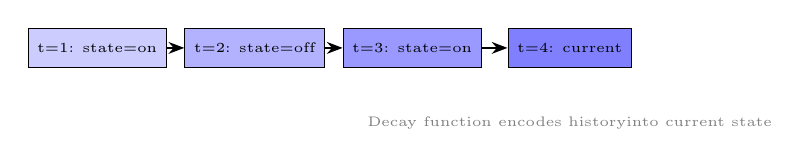
\begin{tikzpicture}[
    timeline/.style={rectangle, draw, minimum height=0.5cm, font=\tiny},
    arrow/.style={-{Stealth[length=2mm]}, thick}
]

\node[timeline, fill=blue!20] (t1) at (0, 0) {t=1: state=on};
\node[timeline, fill=blue!30] (t2) at (2, 0) {t=2: state=off};
\node[timeline, fill=blue!40] (t3) at (4, 0) {t=3: state=on};
\node[timeline, fill=blue!50] (t4) at (6, 0) {t=4: current};

\draw[arrow] (t1) -- (t2);
\draw[arrow] (t2) -- (t3);
\draw[arrow] (t3) -- (t4);

\node[below=0.5cm of t4, font=\tiny, text=gray] {Decay function encodes history\\into current state};

\end{tikzpicture}
\caption{Decay-based self-recording: history emerges from state decay.}
\label{fig:decay}
\end{figure}

The decay function $\delta(t, t_0) = e^{-\lambda(t - t_0)}$ encodes past states into current properties.

\section{Three-Layer Architecture}

\subsection{Architecture Overview}

\begin{figure}[t]
\centering
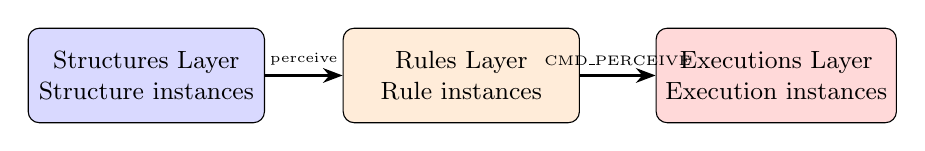
\begin{tikzpicture}[
    node distance=0.8cm and 2cm,
    layer/.style={rectangle, draw, rounded corners=4pt, minimum height=1.2cm, minimum width=3cm, align=center, font=\small},
    arrow/.style={-{Stealth[length=2.5mm]}, thick}
]

\node[layer, fill=blue!15] (structure) at (0, 0) {Structures Layer\\Structure instances};
\node[layer, fill=orange!15] at (4, 0) (rule) {Rules Layer\\Rule instances};
\node[layer, fill=red!15] at (8, 0) (execution) {Executions Layer\\Execution instances};

\draw[arrow] (structure) -- (rule) node[midway, above, font=\tiny] {perceive};
\draw[arrow] (rule) -- (execution) node[midway, above, font=\tiny] {CMD\_PERCEIVE};

\end{tikzpicture}
\caption{LSH Three-Layer Architecture: Structures, Rules, Executions.}
\label{fig:three-layer}
\end{figure}

\subsection{Layer 1: Structures Layer}

The structures layer stores objective properties:

\begin{itemize}
\item Position, size, rotation
\item Physical properties (mass, spectral emission)
\item Relationships (parent-child)
\item Version for change tracking
\end{itemize}

\subsection{Layer 2: Rules Layer}

Observers define perception rules:

\begin{verbatim}
Observer {
    id: observer_id
    rules: Vec<PerceptionRule>
}

PerceptionRule {
    source_category: String
    property_name: String
    compute_type: Direct | Sum | Count | Custom
}
\end{verbatim}

Example: HumanEye observer defines color perception rule:
\begin{equation}
\text{perceived\_color} = \int R(\lambda) \times I(\lambda) \times S(\lambda) \, d\lambda
\end{equation}

where $R(\lambda)$ is spectral reflectance, $I(\lambda)$ is illumination, $S(\lambda)$ is the observer's spectral sensitivity.

\section{Execution Layer}

\subsection{CMD\_PERCEIVE: Perception as Execution}

CMD\_PERCEIVE is the fundamental execution command:

\begin{verbatim}
CMD_PERCEIVE(observer_id, element_id) -> ComputedProperties
\end{verbatim}

Key insight: Perception is \emph{execution}, not \emph{retrieval}. The result is computed from rules, not stored. This has three implications:

\begin{enumerate}
\item \textbf{No storage overhead}: Subjective properties are never stored, only computed on demand
\item \textbf{Automatic consistency}: When objective properties change, perceived properties automatically reflect the change
\item \textbf{Observer-dependent}: Different observers compute different results from the same element
\end{enumerate}

\subsection{Emergent Scheduling}

LSH scheduling emerges from rule-based scoring rather than commanded dispatch:

\begin{equation}
\text{score} = \sum_i \text{rule}_i.\text{score} \times \text{rule}_i.\text{weight}
\end{equation}

Traditional scheduling:
\begin{verbatim}
if GPU_available: assign_to_gpu(task)
elif CPU_available: assign_to_cpu(task)
\end{verbatim}

LSH emergent scheduling:
\begin{verbatim}
score = priority_rule * 0.4 + match_rule * 0.3 + efficiency_rule * 0.3
if score > threshold: execute
\end{verbatim}

\begin{figure}[t]
\centering
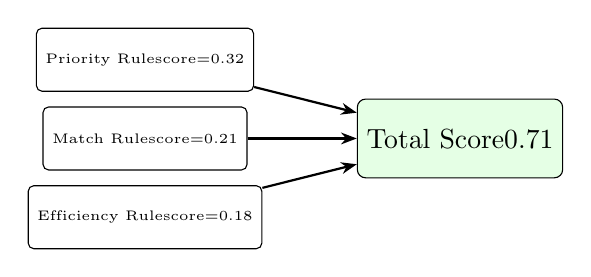
\begin{tikzpicture}[
    rule/.style={rectangle, draw, rounded corners=2pt, minimum height=0.8cm, font=\tiny},
    result/.style={rectangle, draw, rounded corners=3pt, minimum height=1cm, minimum width=2cm, fill=green!10},
    arrow/.style={-{Stealth[length=2mm]}, thick}
]

\node[rule] (r1) at (0, 1) {Priority Rule\\score=0.32};
\node[rule] (r2) at (0, 0) {Match Rule\\score=0.21};
\node[rule] (r3) at (0, -1) {Efficiency Rule\\score=0.18};

\node[result] (total) at (4, 0) {Total Score\\0.71};

\draw[arrow] (r1) -- (total);
\draw[arrow] (r2) -- (total);
\draw[arrow] (r3) -- (total);

\end{tikzpicture}
\caption{Emergent scheduling through rule-based scoring.}
\label{fig:scheduling}
\end{figure}

\subsection{Event-Driven Responsiveness}

Resource changes trigger automatic rescheduling through the view\_sync protocol:

\begin{verbatim}
resource_change -> invalidate() -> cache_clear -> recompute -> new_decision
\end{verbatim}

\subsection{View Synchronization}

The view\_sync protocol provides event-driven updates between the Rust backend and Python/frontend:

\begin{verbatim}
pub enum ViewSyncEventType {
    ElementAdded,
    ElementChanged,
    ElementDeleted,
    ElementPositionChanged,
    SceneActivated,
}
\end{verbatim}

\begin{table}[h]
\centering
\caption{View synchronization event types and triggers.}
\label{tab:view-sync}
\begin{tabular}{lll}
\toprule
\textbf{Event Type} & \textbf{Trigger} & \textbf{Observer Action} \\
\midrule
ElementAdded & New element created & Register for perception \\
ElementChanged & Property updated & Recompute perception \\
ElementDeleted & Element removed & Unregister \\
ElementPositionChanged & Position updated & Update spatial index \\
SceneActivated & Scene switched & Refresh all observers \\
\bottomrule
\end{tabular}
\end{table}

\section{Observer System}

\subsection{Perception Rules}

Observers can define different compute types:

\begin{itemize}
\item \textbf{Direct}: Direct property access
\item \textbf{Sum}: Sum of child element properties
\item \textbf{Count}: Count of elements matching criteria
\item \textbf{Custom}: Arbitrary computation function
\end{itemize}

\subsection{Multi-Observer Perspective}

Different observers perceive the same element differently:

\begin{figure}[t]
\centering
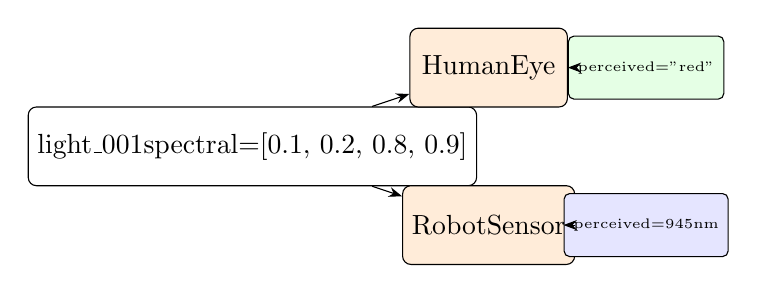
\begin{tikzpicture}[
    node distance=1cm and 1.5cm,
    element/.style={rectangle, draw, rounded corners=3pt, minimum height=1cm, minimum width=2cm},
    observer/.style={rectangle, draw, rounded corners=3pt, minimum height=1cm, minimum width=2cm, fill=orange!15},
    result/.style={rectangle, draw, rounded corners=2pt, minimum height=0.8cm, font=\tiny}
]

\node[element] (light) at (0, 0) {light\_001\\spectral=[0.1, 0.2, 0.8, 0.9]};

\node[observer] (human) at (3, 1) {HumanEye};
\node[result, fill=green!10] (human_result) at (5, 1) {perceived="red"};

\node[observer] (robot) at (3, -1) {RobotSensor};
\node[result, fill=blue!10] (robot_result) at (5, -1) {perceived=945nm};

\draw[-{Stealth}] (light) -- (human);
\draw[-{Stealth}] (light) -- (robot);
\draw[-{Stealth}] (human) -- (human_result);
\draw[-{Stealth}] (robot) -- (robot_result);

\end{tikzpicture}
\caption{Multi-observer perspective: same element, different perceptions.}
\label{fig:multi-observer}
\end{figure}

\section{Implementation}

\subsection{Rust Implementation}

The element model is implemented in Rust:

\begin{verbatim}
pub struct Element {
    pub id: ElementId,
    pub name: String,
    pub category: String,
    pub properties: HashMap<String, serde_json::Value>,
    pub position: Option<[f64; 3]>,
    pub size: Option<[f64; 3]>,
    pub parent_ids: Vec<String>,
    pub children_ids: Vec<String>,
    pub version: u64,
}
\end{verbatim}

\section{Comparison with Related Work}

\begin{table}[h]
\centering
\caption{Comparison with traditional knowledge representations.}
\label{tab:comparison}
\begin{tabular}{lcccc}
\toprule
\textbf{Feature} & \textbf{LSH} & \textbf{RDF} & \textbf{Property Graph} & \textbf{JSON-LD} \\
\midrule
Basic unit & Element & Triple & Node+Edge & Key-Value \\
Structure type & Flat & Graph & Graph & Tree \\
Perception properties & Emergent & Stored & Stored & Stored \\
Observer support & Native & External & External & External \\
History & Decay & Extra storage & Extra storage & Extra storage \\
Scheduling & Emergent & N/A & N/A & N/A \\
\bottomrule
\end{tabular}
\end{table}

\section{Conclusion}

We have presented LSH, a unified world model architecture based on the Element-Observers paradigm:

\begin{enumerate}
\item \textbf{Element Model}: Everything shares common structure
\item \textbf{Three-Layer Architecture}: Structures, Rules, Executions separation
\item \textbf{Observer System}: Rule-based perception computation
\item \textbf{Execution Layer}: CMD\_PERCEIVE, emergent scheduling, and view synchronization
\item \textbf{Decay-Based Self-Recording}: History emerges from state
\end{enumerate}

Future work includes extending the architecture to multi-modal perception and scaling to billion-element scenes.

\bibliographystyle{plainnat}
\begin{thebibliography}{10}

\bibitem[Li(2026a)]{lsh-sfa}
Hengbo Li.
\newblock LSH-SFA: Spacetime Field Attention with Wave Packets, Light-Cone Causality, and PDE-Driven Evolution.
\newblock \emph{LSH Protocol Preprint}, 2026.

\bibitem[Li(2026b)]{lsh-format}
Hengbo Li.
\newblock LSH Format: AI-Native Data Format with Rust/Burn Engineering Validation.
\newblock \emph{LSH Protocol Preprint}, 2026.

\bibitem[Vaswani et~al.(2017)]{vaswani2017attention}
Ashish Vaswani, Noam Shazeer, Niki Parmar, Jakob Uszkoreit, Llion Jones, Aidan~N Gomez, {\L}ukasz Kaiser, and Illia Polosukhin.
\newblock Attention is all you need.
\newblock In \emph{NeurIPS}, 2017.

\end{thebibliography}

\end{document}
